%=====================================================================
\section{From the first certificate towards a delay budget (RQ2, stage 2)}\label{sec:budget}
%=====================================================================
Section~\ref{sec:certificate} ended with a plan: certify the capture controller over the whole spin-up, compute the set of states the drone can be in when the capture controller takes over, and find the largest detection delay for which that set fits inside the certificate. This section carries out the plan step by step and reports what it found. All numbers come from the tables in \texttt{results/tables/} named in each paragraph; every experiment was pre-registered (its fixed choices are written into the script before the first run), and the places where a first attempt had to be changed are listed in Section~\ref{sec:budget-dev}.

\subsection{The chain and the quantities}
The failure unfolds in four phases: the drone starts in some pre-failure set $X_0$; during the \emph{undetected phase} (length $\tau$) the healthy controller keeps flying with rotor 4 at 0\,N; then the published strategy runs the \emph{spin-up} (rotors 1 and 3 at the spin-up thrust, rotor 2 stopped, no feedback) until the body rate exceeds the switch value $w_{\mathrm{sw}}$ (10\,rad/s in the paper); at that moment the failure controller takes over. The states at that moment form the \emph{hand-over set} $S(\tau)$. If a certified capture set $\mathcal C$ contains $S(\tau)$, every start in $X_0$ is guaranteed to be captured. Two numbers summarize the comparison: $\beta(\tau)$, the largest factor by which the shape of $S(\tau)$ can be scaled around its centre and still fit inside $\mathcal C$ ($\beta\ge1$: certified), and $\tau^\star$, the largest delay with $\beta\ge1$. When the centre of $S(\tau)$ is itself outside $\mathcal C$ we report $s_c<1$, the factor by which the centre must be shrunk to reach the boundary of $\mathcal C$. For $X_0$ we use the 99\% ellipsoid of the Gaussian pre-failure distribution of E4 (velocity 0.3\,m/s, attitude 3$^\circ$, body rates 0.3\,rad/s per axis), scaled by a factor $\chi\in\{0, 0.1, 0.25, 0.5, 1\}$; $\chi=0$ is the exact hover. (The scripts and tables call this factor ``gamma''.)

\subsection{Where the hand-over state is (E9a)}
We simulated the published chain for both spin-up thrusts (2.95 and 2.45\,N), $\tau$ from 0 to 130\,ms, and the exact hover plus the 40 pre-failure states of E4 (1312 runs), and recorded the state at the hand-over in the capture coordinates (deviations from the relaxed hover), together with the scaling $s$ of this deviation onto the boundary of the E5 ellipsoid (\texttt{e9a\_handover.md}). The six hover-start rows of Section~\ref{sec:delay} (hand-over time, rates, attitude) were reproduced to two decimals.

\begin{table}[h]
\centering\small
\caption{Hand-over state of the published strategy from the exact hover start (nominal plant) and its position relative to the E5 certificate. $s\ge1$ would mean inside.}\label{tab:e9a}
\begin{tabular}{rrrrrrc}
\toprule
$f_{\text{spin}}$ (N) & $\tau$ (ms) & hand-over (s) & $\Delta r$ (rad/s) & $\|\vect n-\bar{\vect n}\|$ & $s$ & SAFE \\
\midrule
2.95 & 0  & 0.647 & $-8.85$ & 0.75 & 0.232 & yes \\
2.95 & 10 & 0.649 & $-8.93$ & 1.03 & 0.202 & yes \\
2.95 & 20 & 0.649 & $-9.03$ & 1.26 & 0.176 & yes \\
2.95 & 30 & 0.649 & $-9.13$ & 1.43 & 0.157 & no \\
2.45 & 0  & 0.806 & $-8.85$ & 0.66 & 0.271 & yes \\
2.45 & 20 & 0.803 & $-9.02$ & 1.15 & 0.153 & no \\
\bottomrule
\end{tabular}
\end{table}

\paragraph{The hand-over state is far from the hover, even without delay.} At the hand-over the yaw rate is still 9 to 10\,rad/s below its equilibrium value (18.8\,rad/s) and the attitude has tilted by about 0.75 in $\|\vect n-\bar{\vect n}\|$ (Table~\ref{tab:e9a}); with a 20\,ms delay the tilt reaches 1.26, and from $\tau = 45$\,ms (2.95\,N) or 50\,ms (2.45\,N) the drone is upside down at the hand-over ($n_z<0$). The deviation builds up during the open-loop spin-up, not during the delay: with $\tau=0$ the attitude deviation grows from 0.18 to 0.76 between 0.2 and 0.6\,s while the yaw rate climbs (\texttt{e9a\_handover.md}, last table; Figure~\ref{fig:e9a}). The true motor thrusts at the hand-over agree with the failure controller's reset estimate to the printed precision (error 0.00\,N), so the difference between the controller's initial motor estimate and the true thrusts can be neglected for the published chain.

\paragraph{No hand-over state is inside the E5 certificate.} Over all 1312 runs, not one hand-over state lies inside the E5 ellipsoid (neither with all ten states nor with the altitude excluded); the largest $s$ is 0.353 and the smallest 0.062. For the exact hover with $\tau=0$ and 2.95\,N, $s=0.232$. In particular all 374 runs that ended SAFE started their capture \emph{outside} the E5 ellipsoid: the controller recovers from far beyond the certified set, as the nonlinear grid of Section~\ref{sec:certificate} had already shown. This fixes the target of the next steps: the published hand-over state is far outside the first certificate, and so the certificate must be enlarged or the hand-over changed.

\begin{figure}[h]
\centering
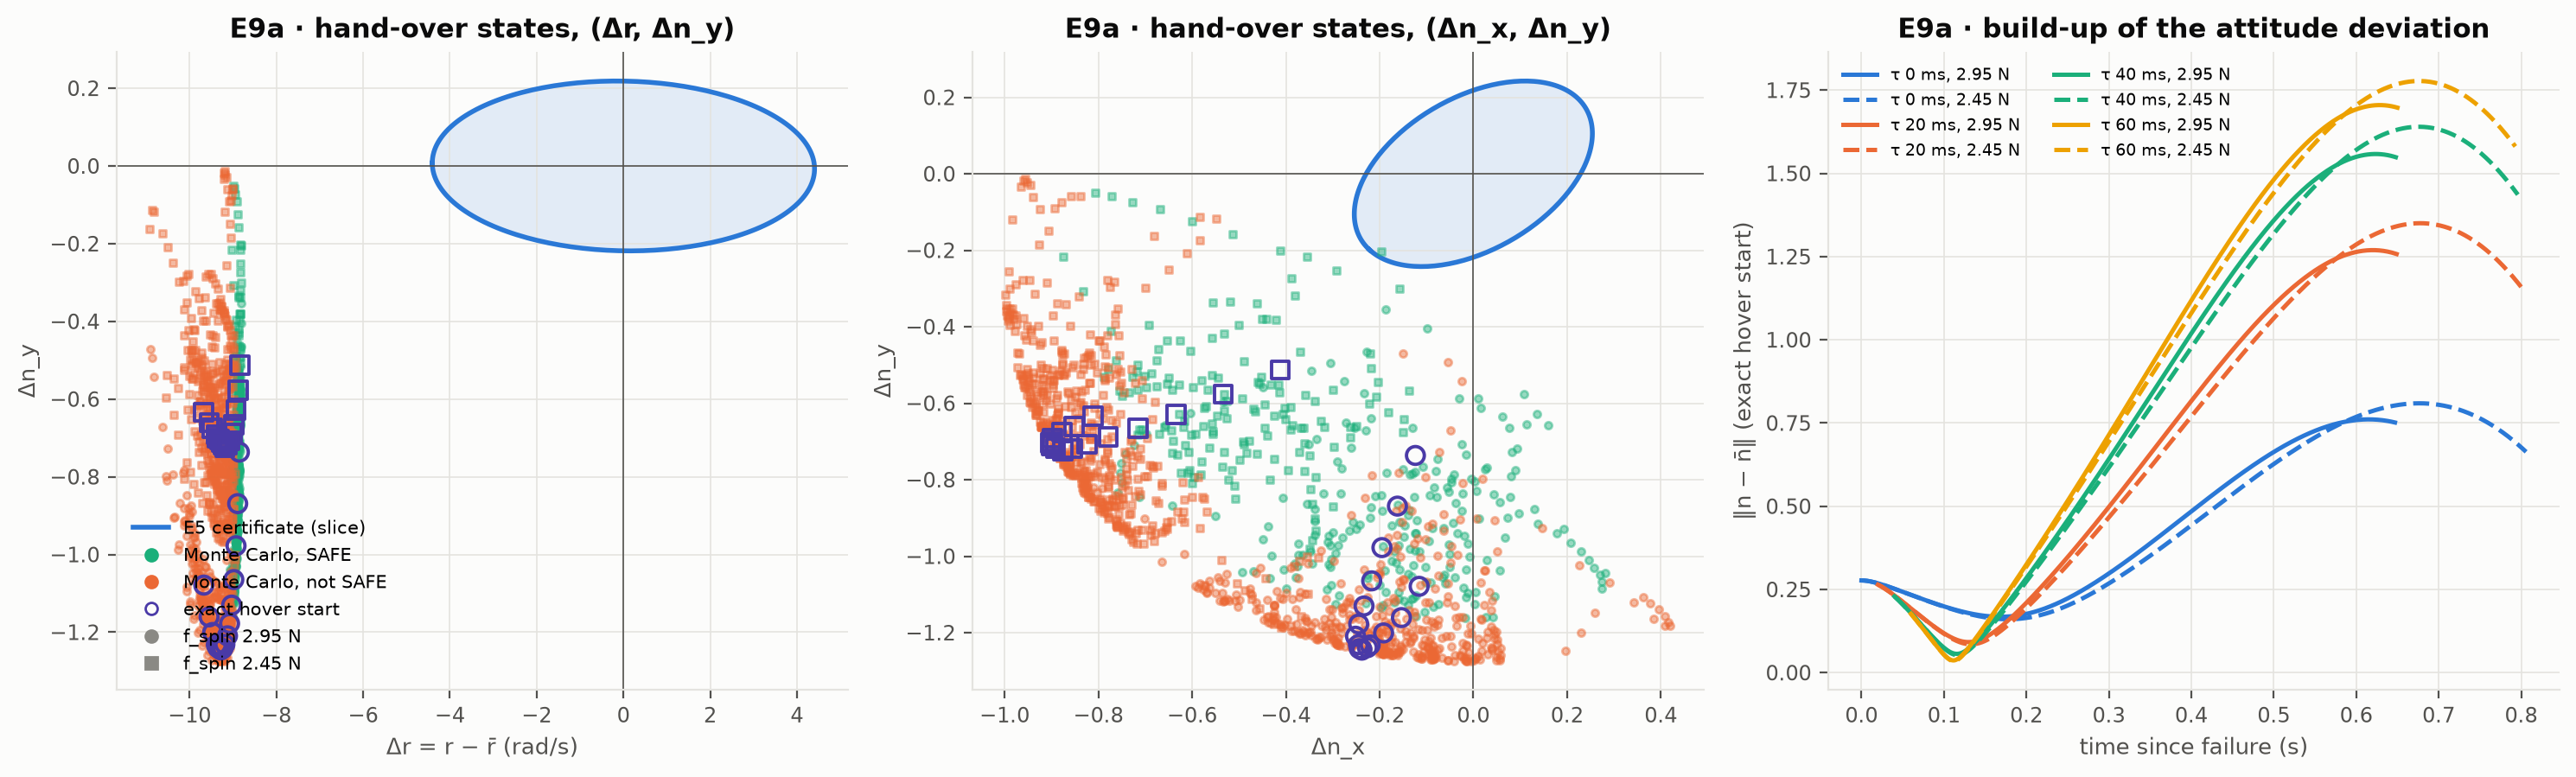
\includegraphics[width=\linewidth]{figures/e9a_handover.png}
\caption{E9a. Left and middle: hand-over states (projected onto $(\Delta r,\Delta n_y)$ and $(\Delta n_x,\Delta n_y)$) of 1312 runs against the slice of the E5 ellipsoid; circles and squares for the two spin-up thrusts, green for SAFE; rings for the exact-hover starts. Right: the attitude deviation during the spin-up for four delays.}\label{fig:e9a}
\end{figure}

\subsection{A certificate that holds over a range of yaw rates (E9b)}
\paragraph{The model.} We replaced the single linearization by a \emph{quasi-linear parameter-varying} (quasi-LPV) model: the closed loop is written as $\dot{\vect e} = A(\vect\vartheta)\vect e + B\operatorname{sat}(-K\vect e) + R(\vect e)$ where the matrix $A$ depends \emph{affinely} on the two scheduling parameters $\vect\vartheta = (r, n_z)$ (the yaw rate and the vertical component of the attitude, both states) and $R$ is a remainder that contains only two small nonlinear effects (the square-root dependence of the propeller speed on thrust, and the dependence of $n_z$ on $n_x,n_y$). The model is implemented in \texttt{rotorfail/lpv.py} and verified against the simulator (the rotational equations to $10^{-10}$, the decomposition to $10^{-10}$, the Jacobian at the trim). The state includes altitude and vertical speed: one might expect that altitude and vertical speed can be left out, but the LQR gain feeds them back into the attitude loop (gain entries of about 1 to 1.5), so the closed loop is not block-triangular. The scheduling box is a family indexed by $\nu$: $r\in[\bar r\pm11\nu]$ and $n_z\in[1-0.8\nu,1]$, with $\nu=1$ covering the hand-over states of E9a with a margin; the failure LQR is stable at every frozen parameter value in the largest box.

\paragraph{The certificate.} For each vertex of the scheduling box and each of the 8 saturation patterns we imposed the Hu--Lin conditions of Section~\ref{sec:certificate} with a common $Q$ (a parameter-dependent matrix was not attempted), in scaled coordinates, with a decay rate of 0.1\,s$^{-1}$, and added two ``self-consistency'' conditions so that the ellipsoid itself implies the parameter range: its projection on $r$ lies inside the box, and its $(n_x,n_y)$ projection lies inside a disc that guarantees $n_z\ge n_{z,\mathrm{lo}}$ (a condition on a box around the hover cannot hold for any ellipsoid that contains the hand-over state, because the hover is off-centre in $n_y$, so the disc form is used). The remainder $R$ was checked after the solve: with $g_P=\max\sqrt{R^\top P R}$ over the boundary of the ellipsoid, the set is invariant with decay at least $2(0.1-g_P)$, so the ellipsoid was shrunk by a factor $\varsigma$ until $g_P\le0.05$ (a numerical estimate by sampling and local optimization, not a proof). Putting the numerical remainder bound into the SDP instead made the certified yaw-rate semi-axis 0.04 to 0.24\,rad/s, so this route was not used.

\begin{table}[h]
\centering\small
\caption{E9b. Largest-volume robust certificates (published LQR, nominal plant) for the scheduling boxes $\nu$. ``Ceiling'' is the largest $\beta$ any hover-centred ellipsoid can reach toward the exact-hover hand-over state because of the disc condition. Final values are after the remainder shrink $\varsigma$; semi-axis in $r$ in rad/s.}\label{tab:e9b}
\begin{tabular}{ccccccc}
\toprule
$\nu$ & $r$ range (rad/s) & verified & ceiling & $\varsigma$ & $r$ semi-axis & $\beta$ to hand-over \\
\midrule
1.0  & 7.81 to 29.81 & no & 0.948 & --- & --- & --- \\
0.8  & 10.01 to 27.61 & yes & 0.885 & 0.0002 & 0.05 & 0.0022 \\
0.6  & 12.21 to 25.41 & yes & 0.780 & 0.0005 & 0.08 & 0.0029 \\
0.4  & 14.41 to 23.21 & yes & 0.618 & 0.001 & 0.08 & 0.0029 \\
0.25 & 16.06 to 21.56 & yes & 0.439 & 0.002 & 0.08 & 0.0027 \\
0.15 & 17.16 to 20.46 & yes & 0.271 & 0.007 & 0.09 & 0.0032 \\
\bottomrule
\end{tabular}
\end{table}

\paragraph{Results.} The certificates for $\nu\le0.8$ pass the independent check required of every LMI result: the worst eigenvalue over all vertices, saturation patterns and a $15\times15$ grid of parameters is $-1.0\times10^{-5}$ in scaled units (the margin $\epsilon$ we asked for), the linear-region blocks are positive semidefinite, and two solvers agree (Clarabel and SCS, objective differing by $1.1\times10^{-3}$ relatively). The solution for $\nu=1$ failed the check (worst eigenvalue $+1.2\times10^{-2}$) and is not used. We then simulated the nonlinear drone from 500 points on the boundary and 500 inside for two of the shrunk certificates ($\nu = 0.15$ and 0.6): none of the 2000 runs left its ellipsoid or failed to be captured. The certified sets are tiny, however: after the remainder shrink the yaw-rate semi-axis is 0.05 to 0.09\,rad/s and the scaling toward the hand-over state is at most 0.0032, against 0.232 for the E5 ellipsoid; and the ceiling column shows that even without the remainder no hover-centred ellipsoid that implies $n_z\ge n_{z,\mathrm{lo}}$ reaches the hand-over state (at most 0.948). The reason is geometric: an ellipsoid centred at the relaxed hover that contains the point $\vect x$ also contains $-\vect x$; the mirror image of the hand-over tilt has $\|(n_x,n_y)\|=1.02>1$, which does not exist. This argument does not depend on the controller, so it also limits the redesign of the next section.

\paragraph{Hypothesis H5 restated.} H5 said that the LTI certificate does not contain the failure state (hover onset) and that a certificate over the spin-up does. The first half was supported (Section~\ref{sec:certificate}); the second half cannot hold as written, because the onset has $r=0$ while this LQR already fails in simulation for $r\le4.8$\,rad/s, so no certificate for this controller can contain it. We therefore restate it as ``a certificate contains the spin-up \emph{hand-over} state'' and keep the original wording above; the outcome of the restated hypothesis is \emph{not supported} for the published LQR: no certificate computed here contains the hand-over state of the published strategy (Table~\ref{tab:e9b}).

\begin{figure}[h]
\centering
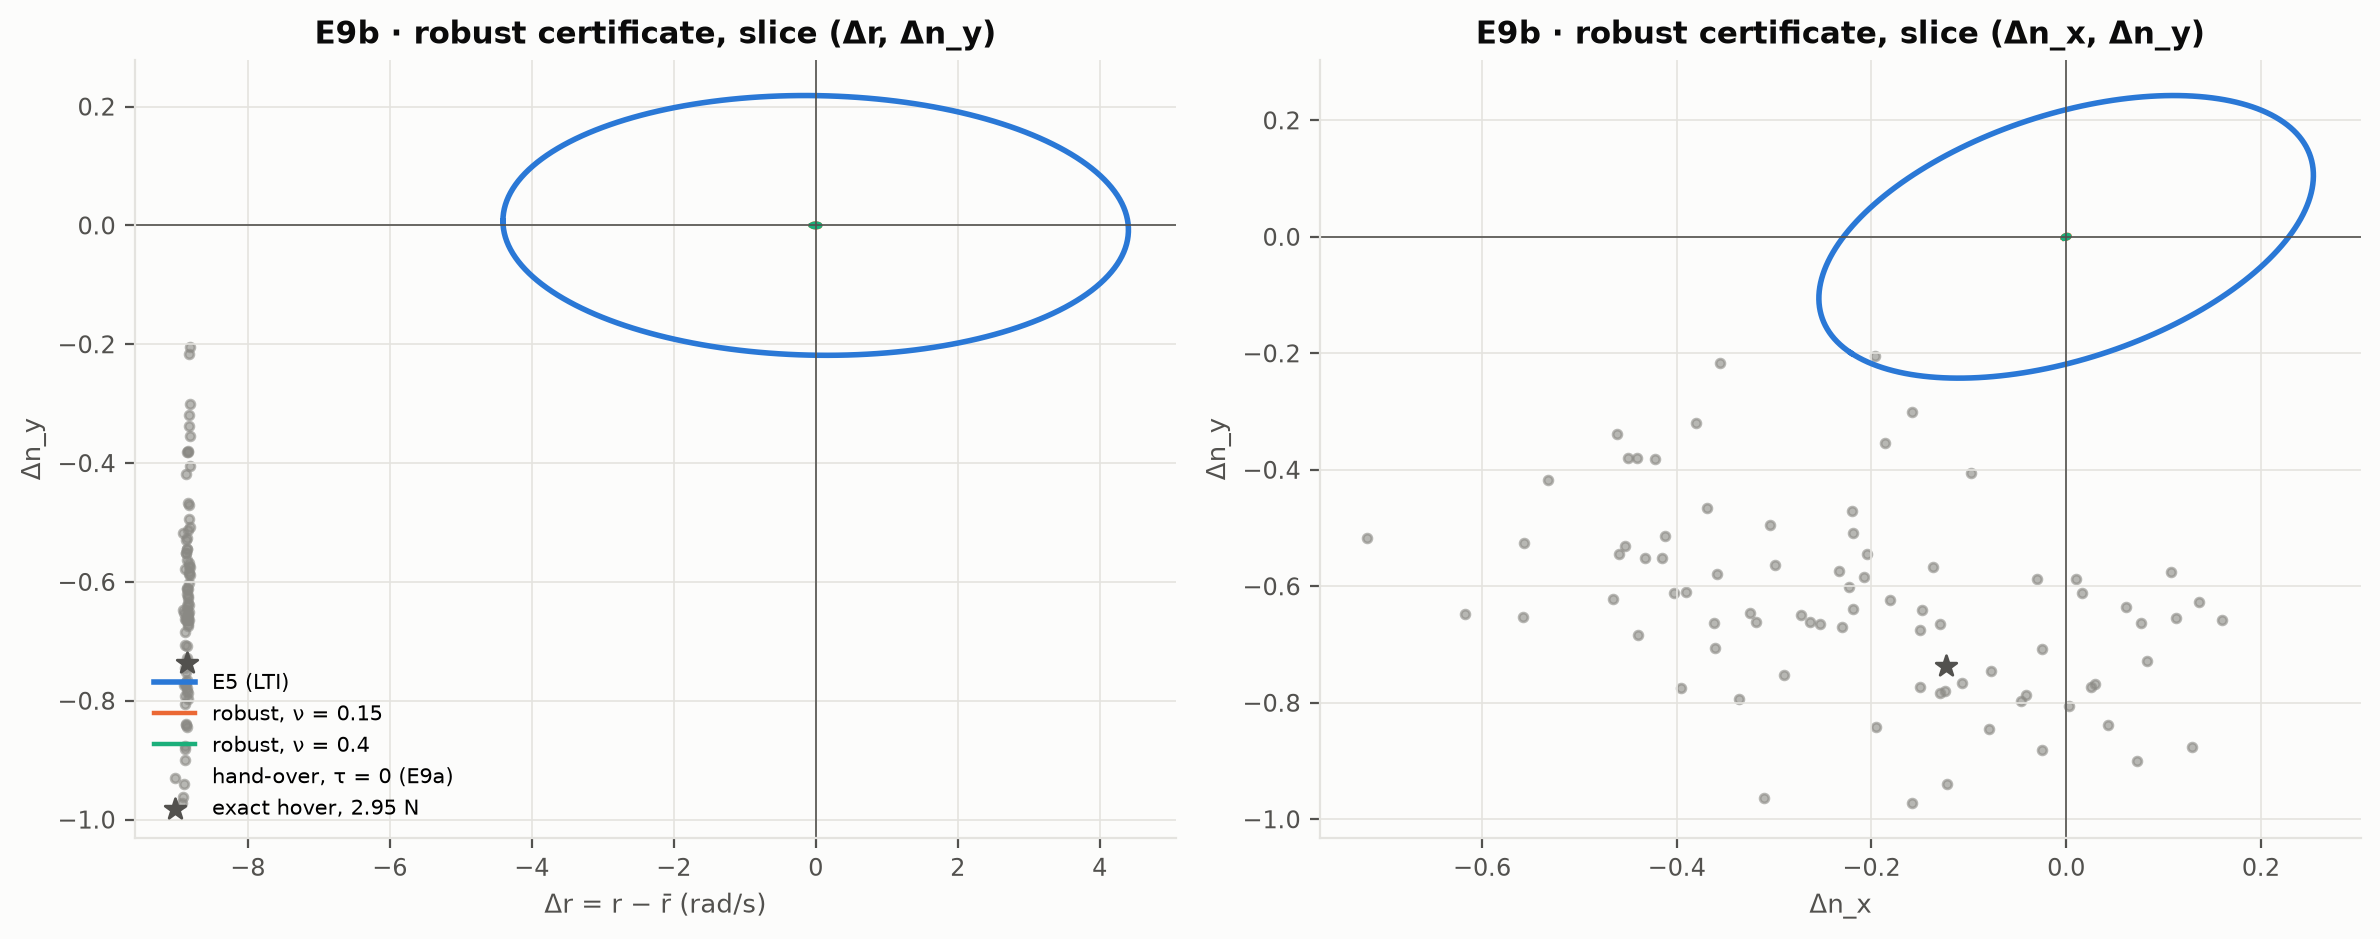
\includegraphics[width=0.95\linewidth]{figures/e9b_robust_certificate.png}
\caption{E9b. Slices of the E5 ellipsoid and of the robust ellipsoids (after the remainder shrink) together with the hand-over states at $\tau=0$ (grey dots) and the exact-hover hand-over state (star).}\label{fig:e9b}
\end{figure}

\subsection{Redesigned capture: a synthesised gain and a different hand-over threshold (E9c)}\label{sec:redesign}
Because no certificate contains the published hand-over state, the framework was used constructively: choose the capture gain \emph{together with} the ellipsoid, by the design form of the Hu--Lin LMIs (variables $Q$, $Y=FQ$ and the auxiliary $Z=HQ$ over all vertices and saturation patterns, plus a bound on the size of the gain over the ellipsoid, $\|F\vect x\|\le g$ for fixed $g\in\{2,4,8,16\}$ in scaled input units), maximizing the extent towards the hand-over state. The hand-over threshold $w_{\mathrm{sw}}$ was varied as well (3, 4, 6, 8, 10, 12, 14, 16, 18\,rad/s), because the spin-up is open loop and its hand-over state does not depend on the gain. Everything produced here is labelled \emph{redesigned capture}; the published strategy (published LQR, $w_{\mathrm{sw}}=10$\,rad/s) is run next to it in every table, unchanged, and the two are never mixed. A synthesised gain is rejected when its closed-loop eigenvalues exceed 100\,rad/s (1.5 times the motor bandwidth; the published LQR has 69\,rad/s) or when the sampled loop is unstable at 1 or 5\,ms. The settings and the rejection rule were fixed before the run (\texttt{results/tables/e9c\_gain\_synthesis.md}).

\paragraph{The hand-over state depends strongly on the threshold.} With a later threshold the yaw rate at the hand-over is close to its equilibrium value but the attitude has tilted for longer; with an earlier one the opposite. The hand-over deviation of the tilt is smallest at 3 and 4\,rad/s (0.17 and 0.21), largest at 10 (0.75; the published value) and 8 (0.66), and the yaw rate deviation runs from $-16.0$ to $-0.8$\,rad/s as the threshold goes from 3 to 18\,rad/s. At every threshold the rotor-2 thrust deviation is $-1.02$\,N and those of rotors 1 and 3 are $+0.91$\,N. The analytic ceiling of the previous section (disc form) is below 1 at 10, 8 and 16\,rad/s (0.80, 0.93, 0.98) and above 1 at the others, so a hover-centred ellipsoid is not excluded there by geometry alone.

\paragraph{Result of the synthesis: no usable gain.} All 36 synthesised designs are feasible and pass the numerical verification (worst eigenvalue $-1.0\times10^{-5}$ in scaled units, the margin requested; the two-solver cross-check on one design differs by 3.0\% and both solves are of reduced accuracy), and the certified extent towards the hand-over state grows over the published LQR gain on the same box: for example 0.46 against 0.31 at 16\,rad/s and 0.20 against 0.15 at 10\,rad/s (remainder-free quasi-LPV certificates). But no design reaches 1, the best being 0.46, and, more importantly, every synthesised gain is unusable: its closed-loop eigenvalues are between 216 and 47\,700\,rad/s (against 69 for the LQR) and the sampled loop is unstable at 5\,ms for 23 of the 36 designs; the other 13 are stable but have eigenvalues of 216 to 453\,rad/s and are rejected by the pole rule. The bound on the gain did not help: the result is the same for $g=2,4,8,16$, because the largest extent is reached by the same ellipsoid in every case. The published LQR gain is verified at all thresholds except 3 and 4\,rad/s (worst eigenvalue $+8\times10^{-2}$) and gives 0.10 to 0.32. After the remainder check only ten designs retain a certificate (certified extents at most 0.0034). So the certified capture of the hand-over state is \emph{infeasible in this framework} for every threshold, gain bound and gain tested: the infeasibility boundary is the interval of extents 0.10 to 0.46 against the required 1.

\paragraph{An earlier hand-over helps in simulation.} Independently of the certificates, the published LQR was simulated with every threshold on 40 new random starts per delay (nominal plant, 2.95\,N; seeds 1000 to 1039, never used for a design) (Table~\ref{tab:thresholds}). The probability of a safe recovery at 20\,ms is 0.65 for the published threshold, 0.72 at 14, 0.80 at 12, 0.88 at 8, and 1.00 at 6\,rad/s, and at 6\,rad/s every start and the exact hover recovered safely up to a delay of 80\,ms (0.97 at 100 and 0.88 at 130\,ms). The effect is not monotone: 18 is slightly worse than 10, and 3\,rad/s fails at every delay including 0\,ms (the hand-over then occurs before the spin has built up), and 4\,rad/s is worse than 6. The best threshold was picked by looking at these seeds, so the statement is confirmed on new seeds and other plants in Section~\ref{sec:pending}.

\begin{table}[h]
\centering\small
\caption{E9c. Empirical delay budget of the published LQR with different hand-over thresholds (nominal plant, 2.95\,N, 40 starts per delay, seeds 1000 to 1039). $\tau_{90}$, $\tau_{50}$: first delay with $P(\text{SAFE})$ below 0.9 and 0.5. Source: \texttt{results/tables/e9c\_gain\_synthesis.md}.}\label{tab:thresholds}
\begin{tabular}{rrrrrr}
\toprule
$w_{\mathrm{sw}}$ (rad/s) & $\tau_{90}$ & $\tau_{50}$ & $P$(SAFE) at 20\,ms & at 60\,ms & at 130\,ms \\
\midrule
10 (published) & 9\,ms & 23\,ms & 0.65 & 0.10 & 0.00 \\
18 & 9\,ms & 20\,ms & 0.50 & 0.03 & 0.00 \\
16 & 9\,ms & 23\,ms & 0.62 & 0.10 & 0.00 \\
14 & 12\,ms & 28\,ms & 0.72 & 0.12 & 0.00 \\
12 & 15\,ms & 33\,ms & 0.80 & 0.20 & 0.00 \\
8 & 15\,ms & 42\,ms & 0.88 & 0.30 & 0.03 \\
6 & $>60$\,ms & $>60$\,ms & 1.00 & 1.00 & 0.88 \\
4 & 17\,ms & 33\,ms & 0.85 & 0.33 & 0.17 \\
3 & 0\,ms & 0\,ms & 0.00 & 0.00 & 0.00 \\
\bottomrule
\end{tabular}
\end{table}

\subsection{Reachable hand-over sets, containment and the delay budget (E9d)}\label{sec:reach}
The last step of the plan is the comparison of the hand-over set $S(\tau)$ with a certified capture set (\texttt{rotorfail/reach.py}, \texttt{results/tables/e9d\_run1\_coverage\_pinv.md}).

\paragraph{Method.} The undetected phase is propagated in two ways. (i) The method of the proposal: an affine linear model of the healthy closed loop with rotor 4 at 0\,N (healthy LQR, sampled at 1\,ms, motor lag), in which an ellipsoid of pre-failure states is propagated exactly (the centre through the augmented matrix exponential, the shape by the transition matrix); it was verified against numerical integration and against 1000 simulated linear trajectories. (ii) A variational method along the nonlinear nominal trajectory: the Jacobian of the whole chain (undetected phase, coordinate change, open-loop spin-up, hand-over at the first controller sample after the crossing, interpolated to the exact crossing for smoothness) with respect to the nine pre-failure variables, by central differences. The saturation of the three working rotors during the undetected phase is classified from the support function of each command over the propagated set (unsaturated, saturated, or ambiguous). Containment of the hand-over ellipsoid in a capture ellipsoid is decided by the S-procedure LMI of Section~\ref{sec:budget} (and independently by an exact trust-region evaluation), for the scale factors $\chi\in\{0,0.1,0.25,0.5,1\}$ of $X_0$, delays up to 130\,ms, both spin-up thrusts, thresholds $w_{\mathrm{sw}}\in\{6,8,10,12,14,16,18\}$\,rad/s, and capture sets from E9c in two tiers: ``rigorous'' (after the remainder check, only the published LQR at 6 and 8\,rad/s) and ``LPV'' (remainder-free, certified for the quasi-LPV model only; the published LQR gain and, for completeness, the rejected synthesised gains).

\paragraph{The undetected phase.} From the exact hover no rotor saturates for $\tau\le60$\,ms (the command of rotor 2 stays above idle), and from $\tau=80$\,ms it is saturated. For the full set $X_0$ ($\chi=1$) the classification is ``ambiguous'' (a rotor may or may not saturate within the set) from the first sample on, for $\chi=0.5$ from 20\,ms, and for $\chi=0.25$ from 60\,ms; in those cases the linear model of the undetected phase is only a local description. The propagated linear ellipsoid contains 98.8\% of 1000 nonlinear samples at $\tau=10$\,ms (largest normalized excess 1.004), 91.7\% at 30\,ms (1.045) and 60.3\% at 60\,ms (1.360): it is a good description for short delays and not for long ones.

\paragraph{Result: the delay budget does not exist.} In all 2560 configurations the \emph{centre} of the hand-over set lies outside the capture set, so the scaling $\beta$ is undefined and $\tau^\star$ does not exist (it would have to be positive at $\tau=0$ already). The scaling $s_c$ that brings the centre onto the boundary is 0.0005 to 0.0018 for the rigorous tier and 0.0027 to 0.461 for the LPV tier. For the published LQR on the published threshold (10\,rad/s) it is 0.147, for the LQR on the best threshold of E9c's empirical study (6\,rad/s) 0.099 (LPV tier) or 0.0017 (rigorous tier), and the largest value of all (0.461) belongs to a synthesised gain that was rejected as not implementable. Because the centre is outside, the size of the scaled set $\chi X_0$ plays no role: the answer is the same for every $\chi$. The altitude loss (the part of the SAFE criterion that the attitude certificate does not bound) is therefore not needed for the conclusion and is observed only in simulation.

\paragraph{What is not in this version.} The first run of this experiment also measured how well the linearised hand-over sets cover nonlinear samples, but that measurement was invalid (a numerical artefact in the pseudo-inverse used for it; the containment results above do not use it); the experiment is being re-run with the corrected measure, and its coverage table is not quoted here.

\subsection{Experiments still running in this version}\label{sec:pending}
Three experiments were still running when this version was written; their results are not quoted anywhere in this report. \emph{E9e} re-tests, on new random starts and on truth families A and B and at the second spin-up thrust, the finding of E9c that the published LQR with a hand-over threshold of 6\,rad/s instead of 10 stayed safe for delays up to 80\,ms (the threshold was picked by looking at the E9c seeds, so it is not yet a confirmed result). \emph{E10a} compares the certified and the empirical delay budget (the certified budget does not exist, so the ratio of the hypothesis H7 cannot be formed; the experiment measures the empirical budget for starts inside $X_0$). \emph{E10b} repeats the study for one parameter at a time (spin-up thrust, idle thrust, healthy tuning, motor time constant, controller period, hand-over threshold).

\subsection{A certificate for the residual Koopman MPC loop (E10c)}\label{sec:mpccert}
The proposal links the two research questions: the residual Koopman MPC should itself get a capture set. Certifying it needs two ingredients, a bound on the learned term and a bound on the true plant mismatch, plus an argument for the MPC constraints. We delivered both as far as they go (\texttt{rotorfail/mpc\_cert.py}, \texttt{results/tables/e10c\_mpc\_certificate.md}).

\paragraph{The unconstrained law.} With the DARE terminal cost and no active input constraint, the MPC (horizon 20, the residual as a constant measured disturbance $\vect d$) is a linear law $\vect u=-K\vect s+G\vect d$ in the 10-state measurement $\vect s=(\vect x,\hat{\vect f})$. $K$ is the LQR gain of the MPC weights; $G$ is the \emph{finite-horizon} feedforward $-K_f(P+\sum_{i=1}^{N-1}(A_{cl}^\top)^iP)$, not the infinite-horizon one (a first version of the code used the latter; the test against the actual QP caught it, and the two now agree to $10^{-5}$\,N at random states). The whole predicted input sequence is then affine in $(\vect s,\vect d)$, so the set where no input bound is active anywhere on the horizon, for every $|\vect d|\le\vect d_{\max}$, is a polytope. The residual is clipped, so $|\hat{\vect d}|\le\vect d_{\max}$ holds by construction (the 99.5\% percentile of the training residuals: 0.101, 0.041, 0.006 for $p,q,r$).

\paragraph{The ellipsoid and the margin.} The largest-volume ellipsoid inside this region that is also contracted by the closed loop (rate $0.995$ per step; the filter states bounded by the thrust range) is verified numerically (worst eigenvalue $-7\times10^{-6}$; face margins within $10^{-11}$); its semi-axes are 0.05 in $n_x$ and $n_y$, 0.96\,rad/s in $r$ and 0.37\,m in $z$. The two-solver cross-check of its volume disagrees strongly (the logarithm of the determinant is $-3.75$ with Clarabel and $+0.19$ with SCS; the SCS solution was not verified), so the set is a verified but possibly suboptimal one; the conclusion below does not depend on its optimality. Robust invariance under the learned term and the true mismatch holds if $\sqrt\lambda+\Delta_{\hat d}+\sum_i\delta_i\|P^{1/2}e_i\|\le1$, with $\lambda=0.995$: the contraction margin is $1-\sqrt\lambda=0.0025$.

\paragraph{Result: the loop cannot be certified.} The learned term alone contributes $\Delta_{\hat d}=1.71$ against the margin 0.0025, so the tolerated plant mismatch is zero. The closed loop is slow (its spectral radius is 0.9946), so a persistent one-step disturbance moves its equilibrium by about 200 times its size, which is the same mechanism as the steady altitude error of Section~\ref{sec:mpc}. The empirical mismatch (1000 runs on 1000 plants drawn from the randomized family, one-step prediction error while the state was inside the ellipsoid) reaches 0.12\,rad/s in $p$ and 0.07\,rad/s in $q$ per step; this is an \emph{empirical} bound, not a proof. With it the left side of the condition is 4.34, so the ellipsoid would have to be about 1335 times larger. The nonlinear check agrees: all 1000 simulated runs (500 from the boundary, 500 from the interior) left the ellipsoid within 3\,s (largest value of the Lyapunov function 60). Finally, the centre of the hand-over set of the published chain lies far outside this capture set: the scaling that brings it onto the boundary is 0.026 at $\tau=0$ and between 0.015 and 0.026 for all delays up to 130\,ms. So the residual MPC gets no certified delay budget; the certificate is conditional, in the same sentence, on a mismatch bound that the data show to be about $10^{3}$ times too large for it.

\subsection{Changes made after first attempts}\label{sec:budget-dev}
For transparency, the places where a first, pre-registered attempt had to be changed (each first run is kept as a separate table in \texttt{results/tables/}; the change was written into the script before the next run):
\begin{itemize}
  \item \textbf{Remainder check of E9b.} The first check bounded the remainder in the Euclidean norm; it failed for every box size and shrink factor because that norm is badly matched to thin ellipsoids (\texttt{e9b\_run1\_euclidean\_check.md}). It was replaced by the bound $g_P$ in the $P$-norm. The shrink-factor grid then ended too early (\texttt{e9b\_run2\_kappa\_grid\_too\_short.md}: $g_P$ scales as $\sqrt{\varsigma}$, so $\varsigma$ of about 0.007 is needed even for the smallest box) and was extended to $10^{-4}$.
  \item \textbf{Discard rule of E8d.} The first rule removed 32 of 40 training episodes because genuine hand-over states already have a tilt deviation of about 0.87 (\texttt{e8d\_run1\_discard\_rule.md}); it was replaced by a divergence rule (non-finite, or body rate above 60\,rad/s).
  \item \textbf{Hand-over search of E9c.} The first launch stopped with an exception before producing any result because the simulation window was too short for thresholds of 14\,rad/s and above; no number was affected.
\end{itemize}
